\documentclass[border=2pt]{standalone}
\usepackage{tikz}
\usetikzlibrary{arrows.meta,positioning,shapes.misc}
\begin{document}
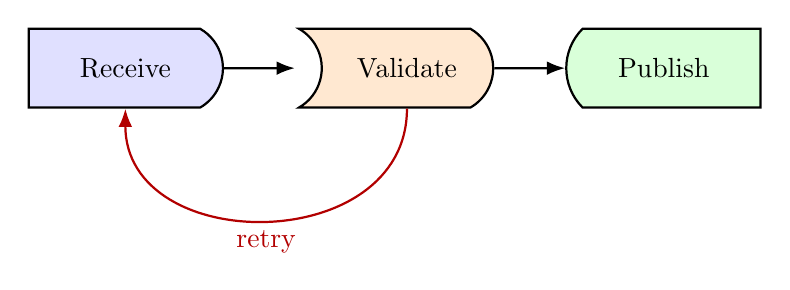
\begin{tikzpicture}[
  >=Latex,
  node distance=9mm,
  every node/.style={draw,rounded rectangle,minimum width=27mm,minimum height=10mm,align=center},
  every path/.style={thick}
]
  \node[fill=blue!12,rounded rectangle west arc=none,rounded rectangle east arc=convex,
    rounded rectangle arc length=120] (input) {Receive};
  \node[right=of input,fill=orange!18,rounded rectangle west arc=concave,
    rounded rectangle east arc=convex,rounded rectangle arc length=120] (check) {Validate};
  \node[right=of check,fill=green!15,rounded rectangle left arc=convex,
    rounded rectangle right arc=none,rounded rectangle arc length=90] (store) {Publish};
  \draw[->] (input) -- (check);
  \draw[->] (check) -- (store);
  \draw[->,red!70!black] (check.south) to[out=-90,in=-90,looseness=1.35]
    node[below,draw=none,fill=none,minimum width=0pt,minimum height=0pt]{retry} (input.south);
\end{tikzpicture}
\end{document}
